\chapter{Implementation}\label{Implementation}
I dette kapitel vil vi beskrive implementeringen af de forskellige dele af løsningsforslaget. Vi har udvalgt nogle forskellige, vigtige dele, af det udviklede program og forklare i dette afsnit hvilken begrundelse til de individuelle dele af programmet og hvilken del det bringer til programmets helhed. Det er ikke alle dele af programmet der er fremhævet i dette afsnit, den fulde kildekode er afleveret sammen med rapporten til eksermination og er ikke dokumenteret i samme større detalje som delene fremhævet i dette afsnit.

\section{Klassediagrammer}\label{Klassediagrammer}
%\externaldocument{appendix}
For at få et overblik over program delene der skulle til for at kunne løse problemet, er der løbende blevet opstillet klassediagrammer. Klassediagrammerne for brugerfladen er ikke vist her, men kan findes i bilag \ref{AppendixA} og \ref{AppendixB}.

\vspace{5mm}

I diagrammerne betyder skråtekst at klassen er abstrakt, plus er et offentligt medlem, og understregning betyder at medlemmet er statisk. Hver klasse har tre kasser, den første indeholder klassens navn, den anden kasse består af klassens fields, og den sidste indeholder klassens properties, metoder og events.

\begin{figure}[H]
    \centering
    \makebox[\textwidth][c]{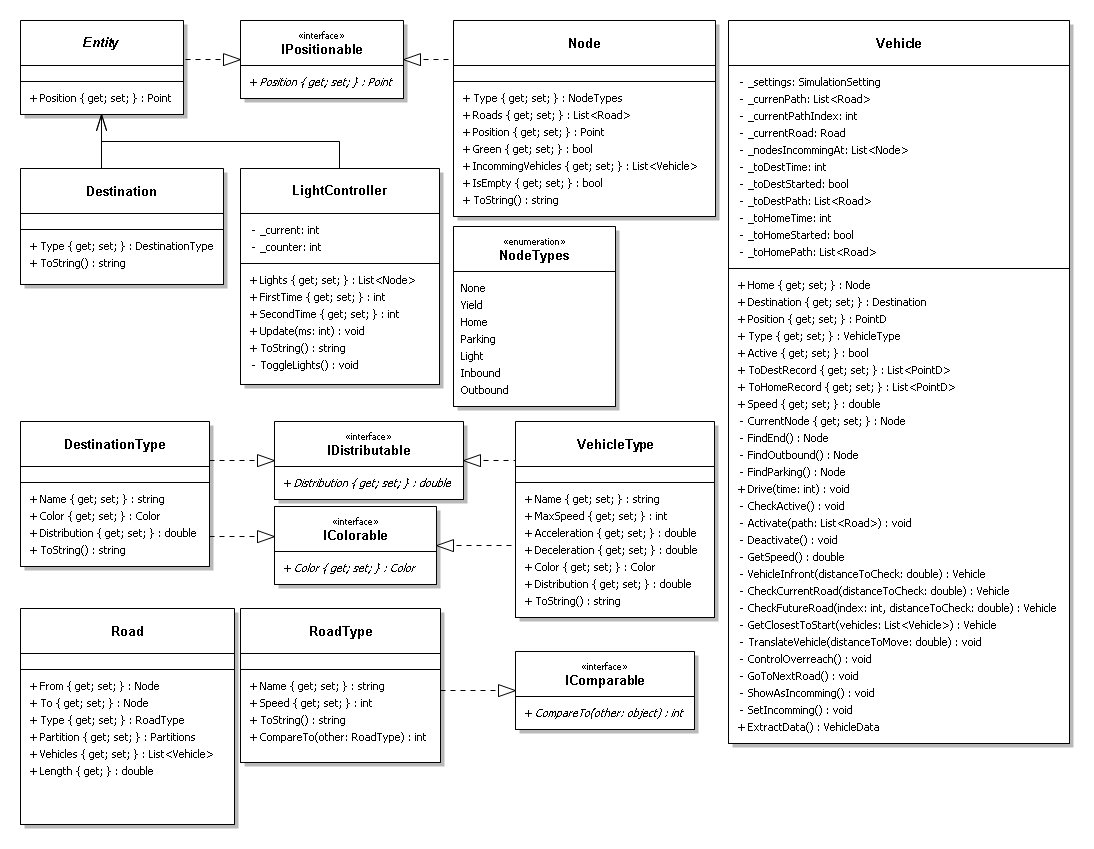
\includegraphics[width=\textwidth,height=\textheight,keepaspectratio]{Pictures/Klassediagram/VejElementer}}
    \caption{Elementer i vejnettet}
    \label{kdVejElementer}
\end{figure}

Diagrammet der ses på figur \ref{kdVejElementer} indeholder alle klasserne der er en del af vejnettet. \texttt{Node} klassen er de knuder vejne kan forbindes imellem. \texttt{Destination} og \texttt{LightControllerne} kan positioneres ligesom \texttt{Node} klassen, men de kan ikke blive forbundet til vejnettet. \texttt{Road} klassen beskriver vejene køretøjerne kan bevæge sig langs. \texttt{Vehicle} klassen beskriver et køretøj, og hvordan hastighed og bevægelsen skal foregå. \texttt{Destination}, \texttt{Road} og \texttt{Vehicle} klasserne har hver især en tilsvarende type-klasse, som brugeren kan lave nye instanser af og dermed bestemme elementernes egenskaber. Elementerne i dette diagram bliver uddybet på i afsnit \ref{ElementerVejnettet}, bortset fra \texttt{Vehicle} der bliver forklaret i afsnit \ref{Vehicle}.

\begin{figure}[H]
    \centering
    \makebox[\textwidth][c]{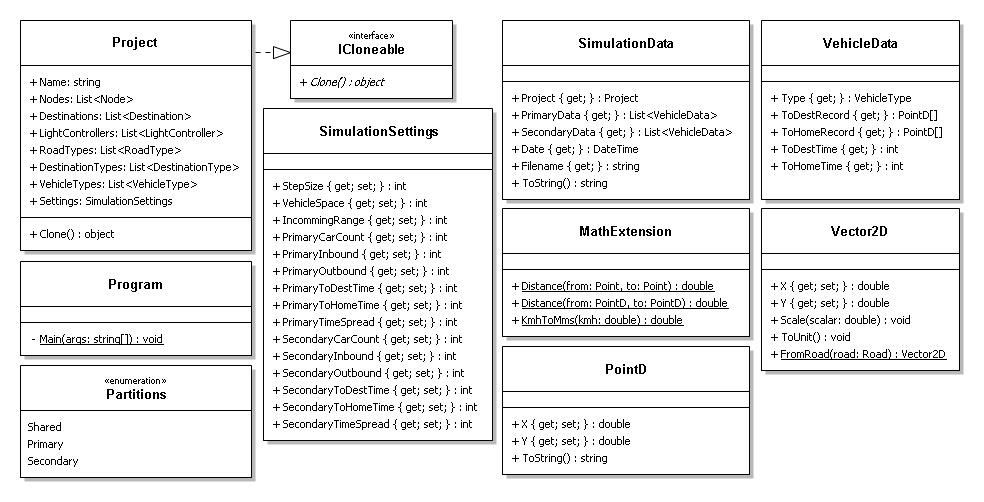
\includegraphics[width=\textwidth,height=\textheight,keepaspectratio]{Pictures/Klassediagram/Diverse}}
    \caption{Diverse klasser}
    \label{kdDiverse}
\end{figure}

På figur \ref{kdDiverse} ses diagrammet for nogle forskellige klasser der ikke ligger under en bred kategori. \texttt{Project} klassen indeholder alt informationen om brugerens indstillinger og brugerens opbyggede vejnet. \texttt{SimulationData} indeholder en klon af projektet fra det tidspunkt det blev simuleret, og en optagelse af den positionelle data fra \texttt{Vehicle} instanserne der befærdede sig på vejnettet. \texttt{Partitions} er en enumerator der bliver brugt forskellige steder gennem programmet til at skelne mellem den primære og den sekundære simulering. \texttt{PointD} er en klasse der beskriver et punkt med doubles, for ikke at miste præcision ved at konvertere mellem floats og doubles. Den statiske klasse \texttt{MathExtension} indeholder nogle formler der ikke findes i standard biblioteket \texttt{Math}. \texttt{Vector2D} beskriver en vektor, og har nogle hjælpe metoder til at arbejde med vektorer. Disse klasser bliver uddybet i afsnit \ref{Diverse}.


\begin{figure}[H]
    \centering
    \makebox[\textwidth][c]{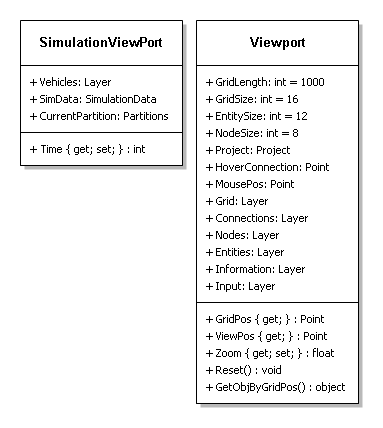
\includegraphics[width=0.4\textwidth,height=\textheight,keepaspectratio]{Pictures/Klassediagram/Viewport}}
    \caption{Viewport og SimulationViewport}
    \label{kdViewport}
\end{figure}

De to klasser på figur \ref{kdViewport} er brugerflade elementerne hvor brugeren kan se vejnettet. Den første klasse \texttt{Viewport}, er den der ses i programmets hoved brugerflade \texttt{GUIMain}, hvor der kan redigeres i vejnettet. Klassen \texttt{SimulationViewport} arver fra Viewport, og bruges til at vise hvordan køretøjerne bevæger sig. Disse klasser forklares i afsnit \ref{HovedBrugerfladen}.

\begin{figure}[H]
    \centering
    \makebox[\textwidth][c]{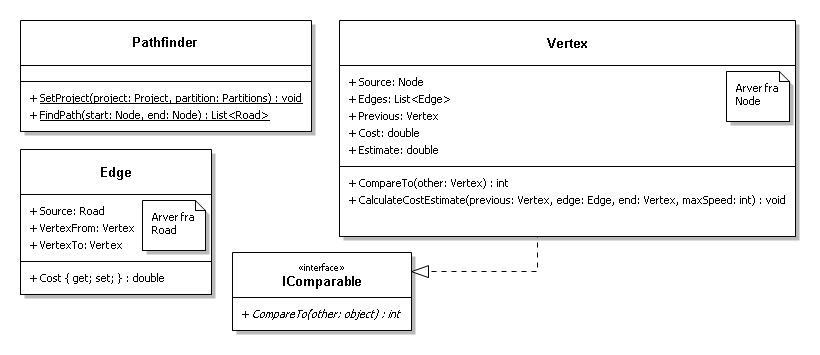
\includegraphics[width=\textwidth,height=\textheight,keepaspectratio]{Pictures/Klassediagram/Pathfinder}}
    \caption{Pathfinder klassen}
    \label{kdPathfinder}
\end{figure}

\texttt{Pathfinder} klassen, som vises sammen med \texttt{Vertex} og \texttt{Edge} klasserne på figur \ref{kdPathfinder}, bruges hver gang en \texttt{Vehicle} bliver konstrueret. Ved \texttt{Vehicle}'s konstruktion, findes den hurtigste vej til destinationen og ruten tilbage igen, som gemmes i selve \texttt{Vehicle} instansen. \texttt{Vertex} og \texttt{Edge} arver fra \texttt{Node} og \texttt{Road}, og indeholder yderligere informationer som \texttt{Pathfinder} bruger til at finde den optimale rute. \texttt{Pathfinder} beskrives i afsnit \ref{Pathfinder}.

\begin{figure}[H]
    \centering
    \makebox[\textwidth][c]{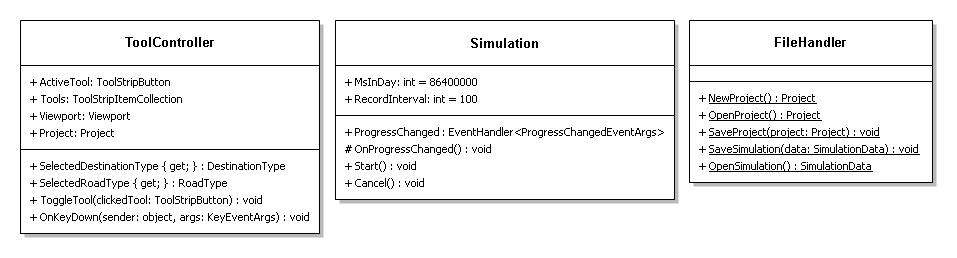
\includegraphics[width=\textwidth,height=\textheight,keepaspectratio]{Pictures/Klassediagram/Funktionalitet}}
    \caption{De funktionelle klasser}
    \label{kdFunktionelle}
\end{figure}

Diagrammet på figur \ref{kdFunktionelle} viser klasserne hvor en stor del af programmets logik bliver håndteret. \texttt{ToolControllerne} modtager input fra \texttt{GUIMain} når der bliver trykket på værktøjsknapperne, og modtager input fra Viewporten når der bliver trykket på gitteret, hvor den så derefter bestemmer hvad der skal ske baseret på det aktive værktøj. \texttt{Simulation} klassen håndterer selve simuleringerne af de primære og sekundære køretøjer, over en periode på 24 timer. \texttt{FileHandler} klassen er statisk og kan gemme og åbne \texttt{Project} klassen og \texttt{SimulationData} klassen. Disse klasser bliver forklaret i afsnit \ref{Kernefunktionalitet}.
\section{GUIMain}\label{HovedBrugerfladen}
Dette afsnit omhandler flowet og indholdet af \texttt{GUIMain}, programmets start og hoved vindue. 

\begin{figure}[!h]
    \centering
    \includegraphics[width=\textwidth,height=\textheight,keepaspectratio]{Pictures/Implementation/program2}
    \caption{Programmets hoved vindue - GUIMain}
    \label{a319program}
\end{figure}

På figur \ref{a319program} ses \texttt{GUIMain}. GUIMain består af en menulinje\textbf(1), værktøjslinje\textbf(2) og en Viewport\textbf(3). Vinduet fungerer udelukkende ved brug af events. Ved tryk på et menupunkt, vil der udløses en event, der åbner det tilsvarende vindue. Menupunkterne er delt op i 4 forskellige kategorier. \texttt{File} indeholder menupunkter der håndtrer fil åbning og gemning. \texttt{Settings} har indstillinger til det nuværende projekt, fordeling af destinationer og transportmiddelvalg, og sidst indstillinger for hvordan simuleringen skal udføres. \texttt{Types} har menupunkter til opsætning af forskellige destination, vej og køretøj typer. Sidst kan man igennem \texttt{Simulation} køre og vise simuleringer.

\vspace{5mm}

Værktøjslinjen har en række knapper der kan tjekkes. Når en knap bliver trykket på, bliver der sendt en event der kalder metoden \texttt{ToggleTool} på \newline \texttt{ToolControlleren}. \texttt{ToggleTool} sørger for at der kun er en aktiv knap ad gangen. Derudover er der to lister på værktøjslinjen, i listen til venstre kan brugeren vælge den \texttt{DestinationType}\textbf(4) der bliver brugt, og i listen til højre kan brugeren vælge hvilken \texttt{RoadType}\textbf(5) der skal bruges.

\vspace{5mm}

\texttt{Viewporten} er gitteret hvor der er muligt at opstille et vejnet. \texttt{Viewporten} abonnerer på \texttt{Move} og \texttt{Click} begivenhederne. Hver gang brugeren flytter musen, vil \texttt{Viewporten} finde ud af hvor musen er, og tegne en cirkel, så brugeren kan være sikker på, hvilken gitter position der vil blive tilføjet til på forhånd. Ved tilfældet at brugeren trykker på \texttt{Viewporten}, tjekker \texttt{ToolControlleren} efter hvilket værktøj der er aktivt, og kører metoden der er forbundet til værktøjet.
\section{Elementerne i Vejnettet}\label{ElementerVejnettet}
\subsection{Node}
I vores program anvender vi et grid hvorpå brugeren indsætter noder der udgør de forskellige vejnet der bliver oprettet. Disse noder kan være forskellige typer. Dette er gjort således at processen i at oprette vejnet er relativt simple. Et simpelt eksempel ville være at brugeren indsætter to noder, den første node hvor brugeren ønsker køretøjerne skal køre fra, og en node med typen \texttt{Parking} tæt på køretøjernes \texttt{Destination}. Således kan et meget simpelt vejnet opstille. Men det er også muligt for brugeren at opstille meget mere komplekse vejnet med lyskryds.

\subsection{Destination}
\texttt{Destination} klassen i vores program er et punkt hvorpå køretøjerne vil søge henimod. Dette er ikke det punkt hvor køretøjerne stopper, til dette formål anvendes der en \texttt{Node} som er angivet til at være til parkering i nærheden af en \texttt{Destination}. \texttt{Destination} klassen består af en instans af \texttt{DestionationType} klassen, dette er, ligesom med \texttt{Vehicle} og \texttt{Road} klasserne, en klasse der bruges til at brugerdefinere forskellige typer af destinations med forskellige parametre.

\subsection{LightController}
\texttt{LightController} klassen er den del af programmet hvori brugeren kan indstille på deres trafiklys noders opførsel.

\begin{figure}[H]
\begin{lstlisting}
public void Update(int ms)
{
  _counter += ms;
  if (_counter > _current)
  {
    if (_current == FirstTime)
      _current = SecondTime;
    else
      _current = FirstTime;
     ToggleLights();
    _counter = 0;
  }
}
private void ToggleLights()
{
  foreach (Node light in Lights)
  light.Green = !light.Green;
}
\end{lstlisting}
\caption{LightController klassen}\label{LightControllerKlassen}
\end{figure}

\texttt{LightControllerens} funktioner er at skrifte trafiklys fra rød til grøn og tilbage igen. Dette er muligt at gøre ved to seperate intervaller sådan at trafiklysene skifter efter forskellige mængder tid. Dette valg blev truffet efter det blev iagtaget at denne samme opførsel ses også på trafikkryds rundt omkring i Aalborg. Dette er idelt hvis brugeren prøver at simulerer et trafikryds hvor den ene vej er mere anvendt en den anden, f.eks. En vej der leder ind i byen fra en motorvej der krydser med en vej der leder ind til mindre boligkompleks.

\subsection{Road}
Road klassen indeholder de variabler der skal anvendes for at kunne beskrive en vej i programmet.

\begin{figure}[H]
\begin{lstlisting}
[Serializable]
public class Road
{
  public Node From { get; set; }
  public Node To { get; set; }
  public RoadType Type { get; set; }
  public Partitions Partition { get; set; }
  public List<Vehicle> Vehicles { get; set; }
  public double Length
  {
    get { return MathExtension.Distance(From.Position, 
                                        To.Position); }
  }   
  public Road(Node from, Node to, RoadType type, 
              Partitions partition)
  {
    From = from;
    To = to;
    Type = type;
    Partition = partition;
    Vehicles = new List<Vehicle>();
  }
}
\end{lstlisting}
\caption{Road klassen}\label{RoadKlassen}
\end{figure}

Road klassen tager imod en instans af \texttt{RoadType} som brugeren selv har defineret via \texttt{RoadType} klassen. På denne måde har brugeren kontrol over hvilken type vej der tale om og hvordan vejen opfører sig i programmet, f.eks. om det er en motorvej. Vejene er programmeret således at brugeren selv kan opstille forskellige kryds, rundkørsler eller andre avanceret afkørsels baner. \texttt{RoadType} er en seperat klasse hvori brugeren give et \texttt{Name} og en \texttt{Speed}, på denne måde definere brugeren selv hvilke typer veje der optræder i deres simulation.

\subsection{Typer}
\section{Diverse}\label{Diverse}

\section{Project}

Project klassen har til formål at sætte de forskellige types klasser op i lister, mens Project (string name) samtidig sætter default values når man laver en ny RoadType, DestinationType eller VehicleType i programmet, hver gang der bliver "addet" noget nyt til de forskellige lister under Types. Project Clones gør det muligt at gemme det man har lavet i en ny fil, som så kan bruges senere såfremt det skal sættes ind andre steder i programmet ved eksempelvis at copy-paste det.

\begin{figure}[H]
\begin{lstlisting} 

{ 
    [Serializable]
    public class Project : ICloneable
    {
        public string Name;
        public List<Node> Nodes = new List<Node>();
        public List<Destination> Destinations = new List<Destination>();
        public List<LightController> LightControllers = new List<LightController>();
        public List<RoadType> RoadTypes = new List<RoadType>();
        public List<DestinationType> DestinationTypes = new List<DestinationType>();
        public List<VehicleType> VehicleTypes = new List<VehicleType>();
        public List<SimulationData> Simulations = new List<SimulationData>();
        public SimulationSettings Settings = new SimulationSettings();
        
        public Project(string name)
        {
            Name = name;
            RoadTypes.Add(new RoadType("Default", 50));
            DestinationTypes.Add(new DestinationType("Default", Color.LightSlateGray) { Distribution = 100 });
            VehicleTypes.Add(new VehicleType("Default", 130, 5, 5, Color.LightSlateGray) { Distribution = 100 });
        }

        public object Clone()
        {
            MemoryStream memory = new MemoryStream();
            BinaryFormatter formatter = new BinaryFormatter();
            formatter.Serialize(memory, this);
            memory.Position = 0;
            return formatter.Deserialize(memory);
        }
    }
}
\end{lstlisting}
\caption{Project.cs}\label{Project}
\end{figure}


\section{SimulationSettings}

SimulationSettings sætter defaultværdierne til de forskellige variabler, og giver brugeren muligheden for at ændre dem og gemme dem med nye værdier i stedet for de predefineret values, skulle man fortryde de selvdefineret values der er blevet sat, kan man altid vælge SetDefault values, ændre ens settings tilbage til de originale default values.

\begin{figure}[H]
\begin{lstlisting} 

{
    [Serializable]
    public class SimulationSettings
    {
        // Shared
        public int StepSize { get; set; }
        public int VehicleSpace { get; set; }
        public int IncommingRange { get; set; }

        // Primary
        public int PrimaryCarCount { get; set; }
        public int PrimaryInbound { get; set; }
        public int PrimaryOutbound { get; set; }
        public int PrimaryToDestTime { get; set; }
        public int PrimaryToHomeTime { get; set; }
        public int PrimaryTimeSpread { get; set; }

        // Secondary
        public int SecondaryCarCount { get; set; }
        public int SecondaryInbound { get; set; }
        public int SecondaryOutbound { get; set; }
        public int SecondaryToDestTime { get; set; }
        public int SecondaryToHomeTime { get; set; }
        public int SecondaryTimeSpread { get; set; }

        // Defaults
        public SimulationSettings()
        {
            StepSize = 100;
            VehicleSpace = 2;
            IncommingRange = 10;
            PrimaryCarCount = 1000;
            PrimaryInbound = 100;
            PrimaryOutbound = 100;
            PrimaryToDestTime = 28800000; // 08:00
            PrimaryToHomeTime = 57600000; // 16:00
            PrimaryTimeSpread = 14400000; // 4h
            SecondaryCarCount = 1000;
            SecondaryInbound = 100;
            SecondaryOutbound = 100;
            SecondaryToDestTime = 28800000; // 08:00
            SecondaryToHomeTime = 57600000; // 16:00
            SecondaryTimeSpread = 14400000; // 4h
        }
    }
}
\end{lstlisting}
\caption{SimulationSettings}\label{SimulationSettings}
\end{figure}

\subsection{Data}
\subsection{MathExtension}
\subsection{Vector2D}
\section{ViewPort}\label{ViewPort}

ViewPort klassen har til formål at sætte rammerne for brugergrænsefladen og området hvori man kan tegne objekter til brug i simuleringen. Klassen arver fra \textbf{WinForms} Panel klasse. Til dette formål er det nødvendigt for ViewPort and være en del af et nyt projekt og derfor instansieres der en nyt projekt og en række parametre set i figur \ref{ViewportParameters}. Readonly variablerne for "GridLength", "GridSize", "EntitySize" og "NodeSize" er størrelserne for de visuelle objekter på Viewporten.

\vspace{5mm}

Der bliver instansieret en variabel af typen "Project" da Viewporten skal kunne repræsentere projektet. "HoverConnection" visualiserer den forbindelse man prøver at lave mellem to objekter. "MousePos" indikerer det aktuelle punkt hvor musen befinder sig i gitteret, selv ved en nedskalering vil den altid finde det samme koordinat. "GridPos" får data igennem en metode der indikerer alle mulige koordinater i gitteret. Dette er brugbart til at finde koordinaterne til objekterne der bliver tegnet i gitteret.

\begin{figure}[H]
\begin{lstlisting}
public readonly int GridLength = 1000;
public readonly int GridSize = 16;
public readonly int EntitySize = 12;
public readonly int NodeSize = 8;

public Project Project;
public Point HoverConnection = new Point(-1, -1);
public Point MousePos = new Point(0, 0);
public Point GridPos { get { return GetGridPos(); } }
\end{lstlisting}
\caption{}
\label{ViewportParameters}
\end{figure}

Som sagt kan ViewPort indikere koordinaterne til indsatte objekter og dette gør den igennem metoden "GetObjByGridPos" som set i figur \ref{ViewportGetObjByGridPos}. Metoden Tjekker for alle Node, LightController og Destination om deres position er lig GridPos. Hvis den har fundet en, så retunere den det fundne objekt.

\begin{figure}
\begin{lstlisting}
public object GetObjByGridPos()
{
   Node node = Project.Nodes.Find(n => n.Position == GridPos);
   if (node != null)
       return node;
   LightController controller = Project.LightControllers.Find(l => l.Position == GridPos);
   if (controller != null)
	   return controller;
   Destination dest = Project.Destinations.Find(d => d.Position == GridPos);
   if (dest != null)
	   return dest;
   return null;
}
\end{lstlisting}
\caption{}
\label{ViewportGetObjByGridPos}
\end{figure}

\input{sections/Implementation/Pathfinder.tex}
\section{Funktionelle}\label{Funktionelle}
%//////////////////////////////// ToolController ////////////////////////////////%
\subsection{ToolController}
\texttt{ToolController} klassen har til formål at forbinde de forskellige værktøjer så når brugeren f.eks. trykker på et af værktøjerne vil \texttt{ToolControlleren} kalde de tilsvarende metoder til værktøjet. Samt at der kun at være valgt et værktøj af gangen. \texttt{ToolController} er altså klassen som står for funktionerne som f.eks. \texttt{AddNode}, \texttt{AddRoad}, \texttt{AddLightController} osv.

\begin{figure}[H]
\begin{lstlisting}
public ToolController(ToolStripItemCollection collection, 
                      Viewport viewport, Project project)
{
   Tools = collection;
   Viewport = viewport;
   Viewport.Input.MouseClick += ViewportClick;
   Project = project;
}
\end{lstlisting}
\caption{ToolController metoden}\label{ToolControllerCode}
\end{figure}

På figur \ref{ToolControllerCode} ses constructoren til \texttt{ToolController}, der bliver kaldt via GUIMain som sender alle værktøjerne, nuværende viewport samt projekt. Herved har \texttt{ToolController} alle elementerne til f.eks at tilføje en \texttt{Node}.

\begin{figure}[H]
\begin{lstlisting}
private void ViewportClick(object sender, MouseEventArgs args)
{
  if (ActiveTool != null && args.Button == MouseButtons.Left)
  {
    switch (ActiveTool.Name)
    {
      ...
      case "ToolAddNode": Add(typeof(Node)); break;
      case "ToolLinkLight": LinkLight(); break;
      case "ToolAddDestination": Add(typeof(Destination)); break;
      case "ToolAddRoad": AddRoad(Partitions.Shared); break;
      case "ToolPrimaryRoad": AddRoad(Partitions.Primary); break;
      case "ToolEdit": Edit(); break;
      ...
    }
  }
}
\end{lstlisting}
\caption{ViewportClick metoden}\label{ViewportClickCode}
\end{figure}

Derudover bliver click eventen på \texttt{Input} lageret af \texttt{Viewporten} i constructoren sat til at blive håndteret af metoden \texttt{ViewportClick}. \texttt{ViewportClick} der kan ses på figur \ref{ViewportClickCode} tjekker hvilket værktøj der er aktivt og kalder den tilsvarende metode.

\begin{figure}[H]
\begin{lstlisting}
public void ToggleTool(ToolStripButton clickedTool)
{
  if (clickedTool.Checked)
  {
    clickedTool.Checked = false;
    ActiveTool = null;
  }
  else
  {
    foreach (ToolStripButton tool in 
      Tools.OfType<ToolStripButton>())
      tool.Checked = false;
    clickedTool.Checked = true;
    ActiveTool = clickedTool;
  }
  StopConnection();
}
\end{lstlisting}
\caption{ToggleTool metoden}\label{ToggleToolCode}
\end{figure}

For at sikre at der ikke er “valgt” flere værktøjer på samme tid, kaldes metoden på figur \ref{ToggleToolCode} \texttt{ToogleTool}, hvergang et værktøj bliver trykket på. Metoden fravælger alle \texttt{ToolStripButtons} i værktøjsListen, hvorefter det nuværende værktøj bliver sat til \texttt{true} (active). Derefter bliver det valgte værktøj sat over i \texttt{ActiveTool} variablen. Til sidst bliver \texttt{StopConnection()} kaldt, som er en metode til at nulstille værktøjets handling, så hvis man f.eks. har valgt \texttt{AddRoad} så vil \texttt{StopConnection()} sikre at det næste klik på gitteret vil tilføje vejens startpunkt og ikke slutpunkt.

\vspace{5mm}

Klassen indeholder som sagt alle værktøjerne og derfor indeholder klassen også en del metoder, derfor vil kun de mest væsentlige værktøjer blive beskrevet.

\begin{figure}[H]
\begin{lstlisting}
private void Add(Type type)
{
  object obj = Viewport.GetObjByGridPos();
  if (obj == null)
  {
    if (type == typeof(Node))
    {
      Project.Nodes.Add(new Node(Viewport.GridPos));
      Viewport.Nodes.Refresh();
    }
    else if (type == typeof(Destination))
    {
      Project.Destinations.Add(new Destination(Viewport.GridPos,  
                                   SelectedDestinationType));
      Viewport.Entities.Refresh();
    }
    else if (type == typeof(LightController))
    {
      Project.LightControllers.Add(new 
        LightController(Viewport.GridPos));
      Viewport.Entities.Refresh();
    }
  }
  else if (obj is Node)
  {
    ((Node)obj).Type = NodeTypes.None;
    Viewport.Nodes.Refresh();
  }
}
\end{lstlisting}
\caption{Add metoden}\label{AddCode}
\end{figure}

\texttt{Add} metoden der ses på figur \ref{AddCode} benyttes til flere værktøjer som f.eks. at tilføje en \texttt{Node}, \texttt{LightController} eller \texttt{Destination}. Udfra typen som bliver sendt fra metodekaldet bestemmes hvilket objekt som skal tilføjes. Hvis den nuværende position i gitteret er en \texttt{Node} bliver \texttt{NodeTypen} sat til \texttt{None} og gitteret vil blive opdateret med \texttt{Refresh()}.

\begin{figure}[H]
\begin{lstlisting}
private void SetNodeType(NodeTypes type)
{
  object obj = Viewport.GetObjByGridPos();
  if (obj is Node)
  {
    if (type == NodeTypes.Light && 
        ((Node)obj).Type == NodeTypes.Light)
      ((Node)obj).Green = !((Node)obj).Green;
    else
      ((Node)obj).Type = type;
    Viewport.Nodes.Refresh();
  }
}
\end{lstlisting}
\caption{SetNodeType metoden}\label{SetNodeTypeCode}
\end{figure}

\texttt{SetNodeType()} som er vist på \ref{SetNodeTypeCode}, benyttes til at give den enkelte \texttt{Node} en type som f.eks. \texttt{Light}, \texttt{Yield}, \texttt{Home}, \texttt{Parking} osv. Metoden modtager en \texttt{NodeType} som bliver bestemt fra \texttt{ViewportClick()}. Hvorefter den checker om objektet på den nuværende position i gitteret er en \texttt{Node}. Hvis det er en \texttt{Node} vil \texttt{NodeTypen} blive sat til den modtaget type. Til sidst vil gitteret blive opdateret med \texttt{Refresh()}.

\begin{figure}[H]
\begin{lstlisting}
private void AddRoad(Partitions partition)
{
 object obj = Viewport.GetObjByGridPos();
 if (obj != null && obj is Node)
 {
    if (_firstNodeConnection)
    {
      _firstNode = (Node)obj;
      _firstNodeConnection = false;
      Viewport.HoverConnection = ((Node)obj).Position;
    }
    else
    {
      _firstNode.Roads.Add(new Road(_firstNode, (Node)obj, 
                               SelectedRoadType, partition));
      if (Control.ModifierKeys == Keys.Shift)
      {
        _firstNode = (Node)obj;
        Viewport.HoverConnection = ((Node)obj).Position;
      }
      else
      {
        _firstNodeConnection = true;
        Viewport.HoverConnection = new Point(-1, -1);
      }
      Viewport.Connections.Refresh();
    }
  }
}
\end{lstlisting}
\caption{AddRoad metoden}\label{AddRoadCode}
\end{figure}

\texttt{AddRoad()} som kan ses på figur \ref{AddRoadCode}, bruges til at tilføje en vej mellem 2 noder, derfor checkes der først om object på den nuværrende positon i gitteret er en node. Hvis det er en node vil der blive checket om \texttt{\_firstNodeConnection} er sket, altså om startpunktet til vejen er blevet valgt. Hvis \texttt{\_firstNodeConnection} er \texttt{true}, betyder det at det ikke er sket, og noden på den nuværrendeposition i gitteret vil blive sat til \texttt{\_firstNode}, og \texttt{\_firstNodeConnection} vil blive \texttt{false}. Det betyder at næste gang brugeren trykker på en node i gitteret vil programmet vide at \texttt{\_firstNode} er blevet sat, og derfor tilføjes der en vej mellem \texttt{\_firstNode} og noden på den nuværrende position i gitteret.

\vspace{5mm}

Hvis brugern holder "Shift" nede imens, vil programmet sætte \texttt{\_firstNode} til den nuværrende \texttt{Node} efter at der er blevet tilføjet en vej, da den \texttt{Node} vil være startpunktet for den næste vej. Det er en implementation som gør det nemmere og hurtigere for brugeren at tilføje veje. 

%//////////////////////////////// FileHandler ////////////////////////////////%
\subsection{FileHandler}
\texttt{FileHandleren} er sat op så at man har mulighed for at lave et ny projekt, åbne og gemme projektet. Der er blevet dannet tre metoder som håndtere de tre valg for brugeren, for at gøre det mest læsevenligt for dem der skal læse koden. \texttt{FileHandler} gør sig brug af \texttt{BinaryFormatter} for at gemme og åbne de forskellige objekter i binær form. Vi startede ud med at bruge \texttt{XMLSerializer}, da vi lavede \texttt{FileHandleren}. Vi stødte ind på nogle problemer da \texttt{XMLSerializer} skulle læse to objekter som har en reference til hinanden, og det skabte en circular reference som var årsagen til vores program crashede på daværende tidspunkt. Ved denne fejl skiftede vi til \texttt{BinaryFormatter}, da den er i stand til at håndtere en circular reference.

\vspace{5mm}

Metoden \texttt{NewProject} er meget simpel, den åbner et vindue med en \texttt{TextBox}, der beder om et navn til det nye projekt. Hvis et navn blev indtastet vil der så blive oprettet et nyt projekt med det navn, og det vil erstatte \texttt{CurrentProject} i \texttt{GUIMain}.

\begin{figure}[H]
\begin{lstlisting}
static public Project OpenProject()
{
  FileStream file = null;
  try
  {
    OpenFileDialog fileOpen = new OpenFileDialog();
    fileOpen.Filter = "TSP Files|*.tsp";
    if (fileOpen.ShowDialog() == DialogResult.OK)
    {
      BinaryFormatter formatter = new BinaryFormatter();
      file = new FileStream(fileOpen.FileName, FileMode.Open);
      return (Project)formatter.Deserialize(file);
    }
    return null;
  }
  catch (Exception e)
  {
    MessageBox.Show("Error: " + e.Message);
    return null;
  }
  finally
  {
    if (file != null)
    file.Close();
  }
}
\end{lstlisting}
\caption{OpenProject metoden}\label{OpenProjectCode}
\end{figure}

Metoden \texttt{OpenProject}, der vises på figur \ref{OpenProjectCode}, kan åbne et eksisterende projekt, når brugeren trykker på Open Project i menuen. Denne metode benytter sig af \texttt{OpenFileDialog}, som ligger under \texttt{System.Windows.Forms}. Koden benytter sig af try-catch-finally, hvor den går ind i try fasen og tjekker om der om brugeren har valgt en TSP fil (traffic simulation project), hvis TSP filen er valgt så vil metoden deserialisere og åbne det gemte projekt op. Sidst vil finally lukke filen, så andre kan komme til.

\begin{figure}[H]
\begin{lstlisting}
static public void SaveProject(Project project)
{ 
  FileStream file = null;
  try
  {
    SaveFileDialog fileSave = new SaveFileDialog();
    fileSave.AddExtension = true;
    fileSave.DefaultExt = "tsp";
    fileSave.Filter = "TSP Files|*.tsp";
    if (fileSave.ShowDialog() == DialogResult.OK)
    {
      BinaryFormatter formatter = new BinaryFormatter();
      file = new FileStream(fileSave.FileName, FileMode.Create);
      formatter.Serialize(file, project);
    }
  }
  catch (Exception e)
  {
    MessageBox.Show("Error: " + e.Message);
  }
  finally
  {
    if (file != null)
      file.Close();
  }
}
\end{lstlisting}
\caption{SaveProject metoden}\label{SaveProjectCode}
\end{figure}

På figur \ref{SaveProjectCode} ses metoden til at gemme et projekt. Igen benytter programmet af en try-catch-finally, hvor programmet i try fasen laver en ny instans af \texttt{SaveFileDialog}, på den måde kan programmet gemme et projekt som man har arbejdet på. Programmet er sat op at den skal gemme projektet som tsp fil (traffic simulation project). Hvis det ikke lykkes, så vil den kaste en exception med fejlen der er sket. Finally fasen vil den så frigøre resourcerne igen.

\vspace{5mm}

\textbf{MANGLER: Noget om åbning og gemning af SimulationData}

%//////////////////////////////// Simulation ////////////////////////////////%
\subsection{Simulation}
\section{Vehicle}\label{Vehicle}
\section{Fejl og mangler i programmet}\label{FejlOgMangler}
Ikke alle programmets kravspecifikationer er blevet implementeret med ønsket effekt. I et af kriterierne ønskes det, at simuleringen også kan foregå med cyklister og fodgængere. Dette er dog ikke tilfældet, programmet simulere kun med køretøjer, så derfor har vi valgt at tage dette med i videreudvikling. Programmet opfylder dog heller ikke ønsket om acceleration og deceleration dvs. programmet bliver mindre realistisk, da dette var en central del af kriterierne. Samtidig var dette også vigtigt fordi VisSims acceleration og deceleration udspillede sig lineær, meningen var at lave en acceleration og deceleration som udspillede sig eksponentielt, da dette var mere realistisk. I tabel \ref{Fejl og mangler} er de følgende fejl og mangler.

%\centering
%\setlength\LTleft{\fill}
%\setlength\LTright{\fill}
\setlength{\LTleft}{-20cm plus -1fill}
\setlength{\LTright}{\LTleft}
\begin{longtable}{| p{0.50\textwidth} | p{0.50\textwidth} |}
	\hline
\textbf{Funktioner} & \textbf{Løsningsforslag} \\
	\hline
Programmet implementere ikke Fodgængere & Skal implementeres på samme måde som køretøjerne, dog skal der lave en knude, der hedder fodgængerfelt. \\
	\hline
Programmet implementerer ikke cyklister & Skal implementeres således der laves en separat cykelsti, som cyklerne kan cykle på. derudover skal vejene ændres, således cyklister og bliver kan være på en vej. \\ 
	\hline
Programmet implementerer ikke acceleration & Step skal ændre sig på en bestemt måde, således at step forøges gradvist ud fra køretøjets acceleration. Derudover holde øje med om der findes et objekt foran den.\\ 
	\hline
Programmet implementerer ikke deceleration & Køretøjerne skal kunne se yield fra en bestemt distance, så de kan nå at decellerere på samme måde som acceleration, bortset fra at de skal kunne bremse i stedet. \\ 
	\hline
Programmets åbne og gemme funktionalitet bruger for meget tid &  Programmets åbne og gemme funktionalitet skal forbedres ved brug af \texttt{Protobuf}. \\ 
	\hline
TimeSpread, ToHomeTime, SetTime og ToDestinationtime skal ændres således brugeren ikke indtaster millisekunder & Det der står i tekstboksen skal ændres så der står klokkeslæt eller timer, derefter skal teksten konverteres til en integer og ganges op. \\ 
	\hline
Programmets skal implementere menneskelig adfærd så bilerne ikke altid kører deres maksimale hastighed på vejene. & Lave en ny klasse \texttt{Driver}, hvor man kan indstille menneskelig adfærd. \\ 
	\hline
Der skal implementeres UnitTest på alle klasser i kildekoden. & Implementer UnitTests. \\ 
	\hline
Viewport går ud over kanterne i højre side og bunden. & Når programmet genererer gitteret, skal den tjekke programvinduets bredde og højde. Samt sørge for at Viewport positionen ikke kommer til at være større end hele størrelsen minus bredden og højden. \\ 
	\hline
Samling og analyse af simuleringens data. & \texttt{SimulationData} skal gemme alt data som simuleringen har, ved at programmet skal kigge på de forskellige positioner. Hvis positionen er lig hinanden så står den stille, ellers skal den måle hastigheden.\\ 
	\hline
Implementere en hjælpeside til information omkring programmets dele. & Lave en hjælpe knappe, som forklarer med tekst, hvordan programmet fungere. \\ 
	\hline
I et lyskryds kan køretøjerne lave u-vendinger. & Der skal laves en ny vej, som man kun må køre ind på fra bestemte knude. \\ 
	\hline 
\caption{Fejl og mangler}\label{Fejl og mangler}
\end{longtable}



\subsection{Optimering af performance}\label{OptimeringAfPerformance}

\textbf{Hastighed} \\
Som sagt har programmet en svaghed når det kommer til performance. For altefter tickraten på simulationen, samt antal af biler osv vil brug af CPU og hukommelse øge markant. Det betyder at hastigheden på simulationen, og åbning af simulationensfilen kan tage fra få sekunder til flere timer alt efter de valgte simulationindstillinger. \\
Der blev lavet en performance profile som vidste at serialize og deserialize af vores simulations fil som tog det meste af simulation/view tiden. Desuden kan programmet ikke åbne filer, hvis de er over 1.2 GB.(\textbf{fordi VS ikke kan håndtere filer over 1.2GB})

\vspace{5mm}

Der blev derfor også kigget på andre metoder at serialize og deserialize simulation filerne istedet for at bruge XML. Der blev fundet frem til Protocol Buffer, og BinaryFormatter som iføgle flere tests siges at være hurtigere end XML \cite{SerializationPerformance}\cite{ComparingThePerformance}\cite{PerformanceTest}. Der blev derfor implementeret BinartFormatter, da det som XML er en del af NET Framework hvilket gjorde det en del nemmere at implementere, samt det understøttede klasser som Point og Color, hvliket Protocol Buffer ikke gjode som startard(Brug surrogate klasser til at konvetere typer som Point, Color til at være kompitabel til Protocol Buffer). Men selvom at BinaryFormatter er hurtigere end XML bliver det stadig overgået af Protocol Buffer som i nogen tests er 12x så hurtig iforhold til BinaryFormatter \cite{PerformanceTest}\cite{Protobuf}, og siden programmet stadig er langtsomt nå det kommer til serialize og deserialize kunne Protocol Buffer midske simulation/view tiden, og afhjælpe med programmet ikke terminere fordi filen enten er for stor, eller tager forlang tid at åbne.

\vspace{5mm}

\textbf{Hukomelses Brug} \\
Dog vil dette ikke afhjælpe på hukommelses forbruget, for at løse dette kunne vi optimere brugen af datatyper f.eks. bruge floats isetdet for doubles, hvliket vil halvere brugen af hukomelse hvergang vi beytter en double. Vi bruger f.eks double ved vores grid hvor vi bruger points med doubles værdier. \\

En anden måde at løse hukomelses problemet på, er ved brug af Memory-Mapped Files klassen, da den vil kunne splite filen op i en bestemt mægnde bytes  både ved gemning/indlæsning. Herved vil programmet ikke gemme/indlæse hele simulations filen på hukomelsen på engang, men kun den mægnden bytes som Memory-Mapped streamen er sat til. Herved ungåes det at programmet alt efter størelsen på simulationen har et hukommelses forbrug på måske over 4000MB, hvliket i sidste ende vil terminere enten programmet eller computeren.

\vspace{5mm}

\textbf{CPU forbrug} \\
For at optimere CPU forbruget, vil en mulig løsnig være at få GPU'en til at tegne grafikken i programmet, istedet for CPU'en. Dette kan gøres ved brug af Windows Presentation Foundation (WPF). Fordelen ved dette er at den mægnde CPU som bliver sparet,  vil kunne bruges på simulationen istedet, samt er GPU'en hurtigere til at tegne grafik end CPU'en. Derudover vil implemitering af flere "threads" kunne udnytte flere kerner i computeren, og herved øge simulationshastigheden, da vores program kun indeholder 2. Hvliket vil sige at f.eks. på en core i7 maskine med 8 kerner vil kun 25\% kraft blive brugt.






